\documentclass[11pt]{article}

\newcommand{\cnum}{CM146}
\newcommand{\ced}{Fall 2018}
\newcommand{\ctitle}[3]{\title{\vspace{-0.5in}\cnum, \ced\\Problem Set #1: #2}}
\usepackage{enumitem}
\usepackage{graphicx}
\graphicspath{{/home/scott/Documents/Github/Machine_Learning/HW_2}}
\newcommand{\solution}[1]{{{\color{black}{\bf Solution:} {#1}}}}
\usepackage[usenames,dvipsnames,svgnames,table,hyperref]{xcolor}

\renewcommand*{\theenumi}{\alph{enumi}}
\renewcommand*\labelenumi{(\theenumi)}
\renewcommand*{\theenumii}{\roman{enumii}}
\renewcommand*\labelenumii{\theenumii.}


\begin{document}
\ctitle{2}{Perceptron and Regression}
\author{Chaojie Feng}
\date{Oct.25, 2018}
\maketitle
\vspace{-0.75in}

\section{Problem 1}
\solution{Please see CCLE for solution}
\section{Problem 2}
\solution{Please see CCLE for solution}
\section{Problem 3}


\begin{enumerate}
\item Problem 3a

\solution{Assume there is an optimal solution $\delta$ for linear program in equation (2), $\delta$ must be 0 in order for at least one inequalities in (2) to satisfy equality conditions, and leaves the other inequality as before. As a result:

$$ y_i(w^Tx + \theta) \geq 1 $$

Obviously, this equation can be reformatted as: 

\[ 
\bigg \{
  \begin{tabular}{ccc}
  y = 1 if $w^Tx + \theta \geq 1$\\
  y = -1 if $w^Tx + \theta \leq -1$\\
  \end{tabular}
\] 

Its constraint is more relaxed compared to the condition of separability in equation (1). So we can say the dataset is linear separable

}

\vspace{2cm}
\item Problem 3b

\solution{If $0 \leq \delta < 1$ then $D$ is separable. If $\delta = 1$ then the minimal separating margin will be 0. If $\delta > 1$ then $D$ is not separable. As a result, there may be many cases for $\delta > 0$}

\vspace{2cm}
\item Problem 3c

\solution{The optimal solution is $\delta = 0$, which is equivalent as formulation (2). However, this formulation doesn't leave a margin. To be specific, it will give trivial solutions if a point lies on the separating hyperplane (i.e. the margin between dataset $\gamma$ is 0) because $y_i(w^Tx_i + \theta)\geq 0$ holds for both positive and negative cases}

\vspace{2cm}
\item Problem 3d

\solution{The optimal solution will be $\delta = 0$. Also with $ y_i(w^Tx_i + \theta) \geq 1-\delta $:

$$ 1([w_1 \ w_2 \ w_3][1 \ 1 \ 1]^T + \theta) \geq 1 $$
$$ -1([w_1 \ w_2 \ w_3][-1 \ -1 \ -1]^T + \theta) \leq -1 $$
$$ w_1 + w_2 + w_3  \geq 1 +  | \theta | $$
}


\end{enumerate}

\newpage

\section{Problem 4}
\begin{enumerate}

	\item Problem 4a \newline
	
	\solution{
	
	\begin{figure}[h!]
	\centering
	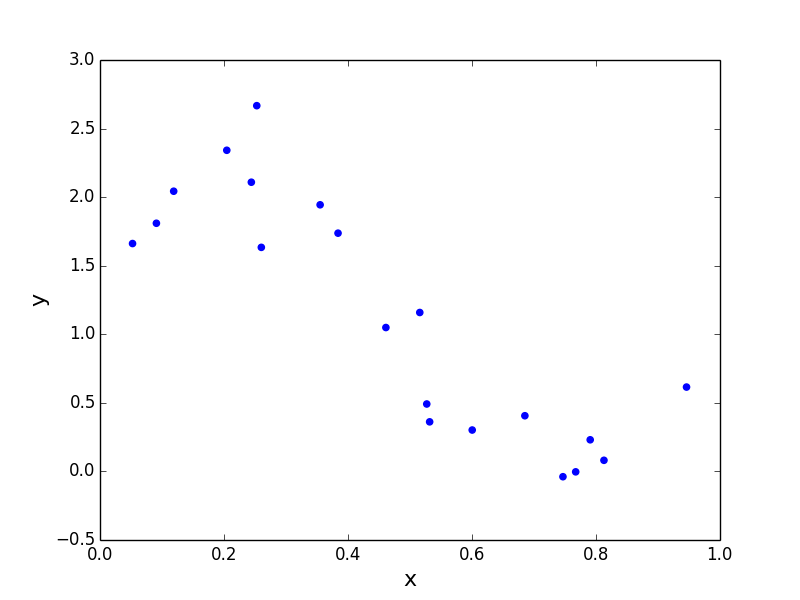
\includegraphics[width = 10cm]{4a}
	\caption{Visualization of training data}
	\end{figure}
	
	From the visualization of training data, a linear regression model will not behave well because
	the trend of data is non-linear. Underfitting will occur if a linear model is chosen 
	
	}
	\vspace{2cm}
	
	\item Problem 4b \newline
	
	\solution{
	
	\begin{figure}[h!]
	\centering
	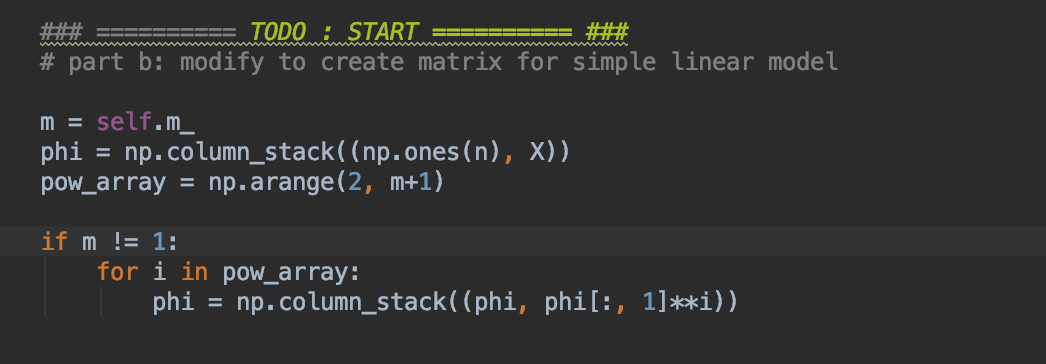
\includegraphics[width = 10cm]{4b}
	\caption{Modified for polynomial feature}
	\end{figure}

	
	}
	\vspace{2cm}
	
	\item Problem 4c \newline
	
	\solution{
	
	\begin{figure}[h!]
	\centering
	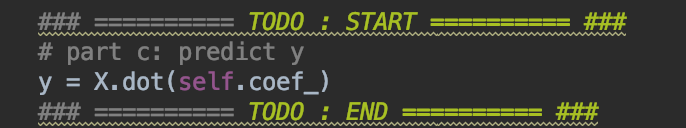
\includegraphics[width = 10cm]{4c}
	\caption{Prediction function}
	\end{figure}
	
	
	}
	\vspace{2cm}
	
	\item Problem 4d \newline
	
	\solution{
	
	\begin{figure}[h!]
	\centering
	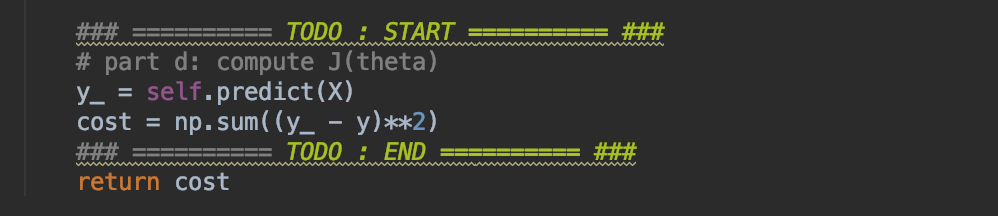
\includegraphics[width = 10cm]{4d}
	\caption{Calculation of cost}
	\end{figure}
	
	\begin{figure}[h!]
	\centering
	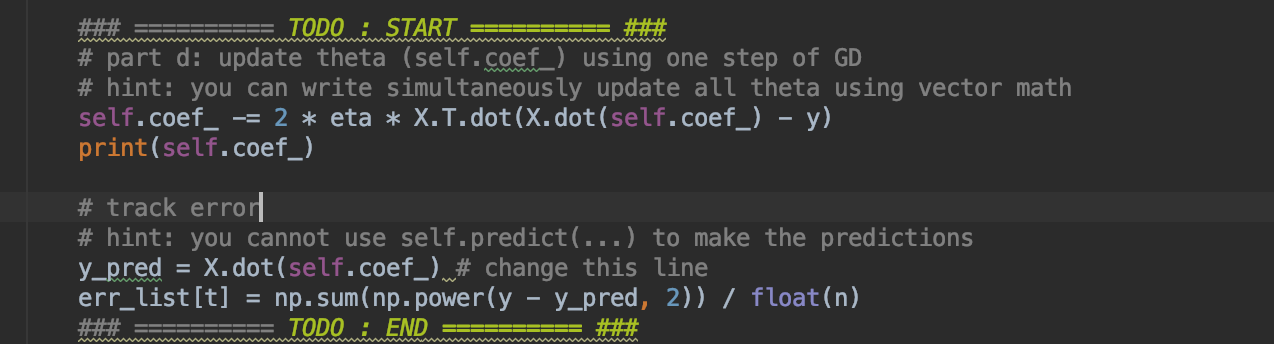
\includegraphics[width = 10cm]{4d2}
	\caption{Gradient descent}
	\end{figure}
	
	\begin{table}[h!]
	\caption{Parameters for gradient descent}
	\begin{center}
 	\begin{tabular}{||c c c c||} 
	 \hline
 	$\eta$ & iterations & J*  & $ \theta $ \\ [0.5ex] 
 	\hline\hline
 	$10^{-4}$ & 10000 & 4.0863 & $[2.2704, -2.4606]$\\ 
 	\hline
 	$10^{-3}$ & 7076 & 3.9126 & $[2.4464, -2.8163]$\\
 	\hline
 	$10^{-2}$ & 765 & 3.9126 & $[2.4464, -2.8163] $\\
 	\hline
 	0.047 & 1000 & $2.711e{39} $ & $[-9.4e18, -4.65e18]$ \\ [1ex]
 	\hline
	\end{tabular}
	\end{center}
	\end{table}
	
	Figure 4, figure 5 and table 1 represent the algorithm for gradient descent as well as their performance. As we can see that if we tune our learning rate $\eta$ to be very small, the GD algorithm will not converge to its global optimal within maximum iteration. If we tune our learning rate to be larger, we can achieve our global optimal, but number of iterations may vary greatly based on different $\eta$. If we tune our learning rate to be too large, we might not be able to converge our GD algorithm to global optimal.
	
	
	
	}
	
	\vspace{2cm}
	
	\item Problem 4e
	
	\solution{
	
	\begin{figure}[h!]
	\centering
	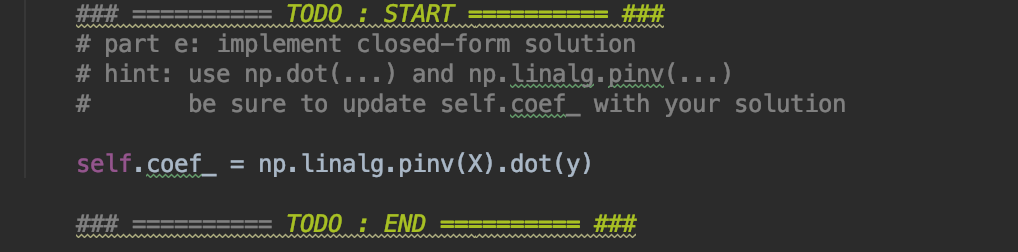
\includegraphics[width = 10cm]{4e}
	\caption{Closed form solution}
	\end{figure}
	
	
		The closed form solution is actually the least square solution for this model, and since our cost is defined as squared loss, the cost will be minimized when $\omega$ achieves optimal value, which will be the same as using gradient descent method. The cost using closed-form solution is 3.9126 and the coefficients $\theta$ is $[2.4464, -2.8163]$. In this case, closed form solution runs faster because the number of features are not large. As number of features increases, the computational cost for closed-form solution will be more expensive than gradient descent.
	
	}
	
	\vspace{2cm}
	
	\item Problem 4f \newline
	
	\solution{
	If we set $\eta$ to be a function of k, It takes 2113 iterations for the algorithm to converge the cost to the same value as closed form solution.
	
	}
	
	\item Problem 4g
	
	\solution{
	Please refer to Problem 4b
	}
	
	\item Problem 4h
	
	\solution{
	From the equation, RMSE includes sample size into calculation. As a result, it is a more comparable and universal metric for the model with different data size. It also scales the error so that it matches with predictions.
	}
	
	
	\vspace{2cm}
	
	\item Problem 4i
	
	\solution{
	
	\begin{figure}[h!]
	\centering
	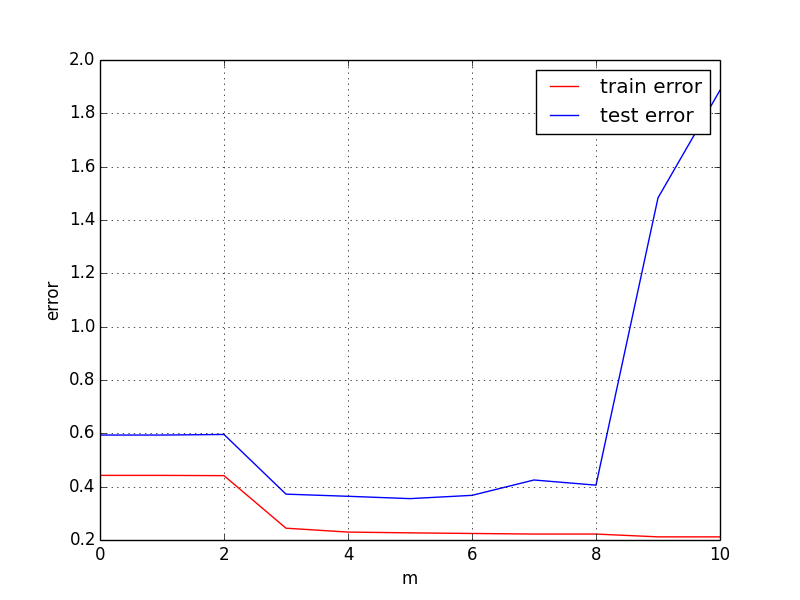
\includegraphics[width = 10cm]{4i}
	\caption{Comparison between training and testing error for m = 1 to 10}
	\end{figure}
	
	From the figure, we can see that if m < 3, the model is underfitting because the training error is high, and when m > 8 the model is overfitting because although training error is nearly zero but testing error is high. As a result, from the figure, the best m is 5
	
	}
	
	
	
	
	
	
	
	
	

\end{enumerate}

\end{document}
